\documentclass[twoside,10pt]{article}
\usepackage{amsmath,amsfonts,amsthm,fullpage,amssymb}
%\usepackage{mymath}
\usepackage{algorithm,amsmath,amssymb}
\usepackage{algorithmic}
\usepackage{graphicx}
\usepackage{url}
\usepackage[most]{tcolorbox}


\begin{document}


\title{ISYE 6740 Homework 5\\ 
Fall 2020\\
\small Total 100 points + 10 bonus points.}
\author{Shasha Liao}
%\date{Deadline: Feb. 13, Sat., 11:55pm}
\date{}
\maketitle



%As usual, please submit a report with sufficient explanation of your answers to each the questions, together with your code, in a zip folder.

%----------------------------------------------------------------------------------



\begin{enumerate}


\item{\bf SVM. } (45 points)

\begin{enumerate}
\item (5 points) Explain why can we set the margin $c = 1$ to derive the SVM formulation?
\begin{tcolorbox}[breakable, enhanced]
\textbf{Solution:} We will prove the equivalence between the following two optimization problems.
\begin{align}\label{eq1}
\begin{split}
\max_{w,b} & \frac{2c}{\|w\|}\\
\text{subject to } & y^i(w^Tx^i + b) \geq c, \forall i.
\end{split}
\end{align}

\begin{align}\label{eq2}
\begin{split}
\max_{w,b} & \frac{1}{\|w\|}\\
\text{subject to } & y^i(w^Tx^i + b) \geq 1, \forall i.
\end{split}
\end{align}

Suppose $w^*, b^*$ are solutions to \eqref{eq1}.
Then we know that for all $w, b$ satisfying $ y^i(w^Tx^i + b) \geq c, \forall i$, we have $$\frac{2c}{\|w\|} \leq \frac{2c}{\|w^*\|},$$ i.e., $$\frac{1}{\|w/c\|} \leq \frac{1}{\|w^*/c\|}.$$ Now let $\hat{w} = w/c, \hat{b} = b/c, \hat{w}^* = w^*/c, \hat{b}^* = b^*/c$, we have 
$$\frac{1}{\|\hat{w}\|} \leq \frac{1}{\|\hat{w}^*\|}$$ for all $\hat{w}, \hat{b}$ satisfying $y^i(\hat{w}^Tx^i + \hat{b}) \geq 1, \forall i$. 
This shows $\hat{w}^*, \hat{b}^* $ are solutions to \eqref{eq2}. Similarly, given any solutions to \eqref{eq2}, we can construct solutions to \eqref{eq1} by scaling. So, problem \eqref{eq1} and \eqref{eq2} are equivalent. 
\end{tcolorbox}

\item (10 points) Using Lagrangian dual formulation, show that the weight vector can be represented as
\[
w = \sum_{i=1}^n \alpha_i y_i x_i.
\]
where $\alpha_i \geq 0$ are the dual variables. What does this imply in terms of how to relate data to $w$?
\begin{tcolorbox}[breakable, enhanced]
\textbf{Solution:} The Lagrangian function is $$L(w,b,\alpha) = \frac 1 2 w^T w + \sum_{i=1}^m \alpha_i (1- y_i (w^Tx_i + b)).$$ Taking derivative and set to zero gives $$\frac{\partial L(w,b,\alpha)}{\partial w} = w - \sum_{i=1}^m \alpha_iy_i x_i = 0. $$ Therefore, $$w = \sum_{i=1}^m \alpha_iy_i x_i.$$ This tells us that the weight vector is a linear combination of the feature vector of the data points.
\end{tcolorbox}

\item (10 points) Explain why only the data points on the ``margin'' will contribute to the sum above, i.e., playing a role in defining $w$. 
\begin{tcolorbox}[enhanced, breakable]
\textbf{Solution:} By the KKT conditions, we need to require that $$\alpha_i (1- y_i (w^Tx_i + b)) = 0, \forall i = 1, 2, ..., m.$$ Since $$1- y_i (w^Tx_i + b) \left\{ \begin{array}{lcr} = 0 & \mbox{ if } x_i \mbox{ is on the margin.} \\
< 0 &\mbox{ otherwise.} \end{array} \right.$$ We have $$\alpha_i  = 0  \mbox{ if } x_i \mbox{ is not on the margin.} $$ Therefore, in the sum $w = \sum_{i=1}^m \alpha_iy_i x_i$, all the terms corresponding to data points not on the margin will disappear and we are only left with the terms corresponding to data points on the margin, which are called the support vectors. 
\end{tcolorbox}

\item (20 points) Suppose we only have four training examples in two dimensions as shown in Fig. The positive samples at $x_1 = (0, 0)$, $x_2 = (2, 2)$ and negative samples at $x_3 = (h, 1)$ and $x_4 = (0, 3)$. 
%
\begin{center}
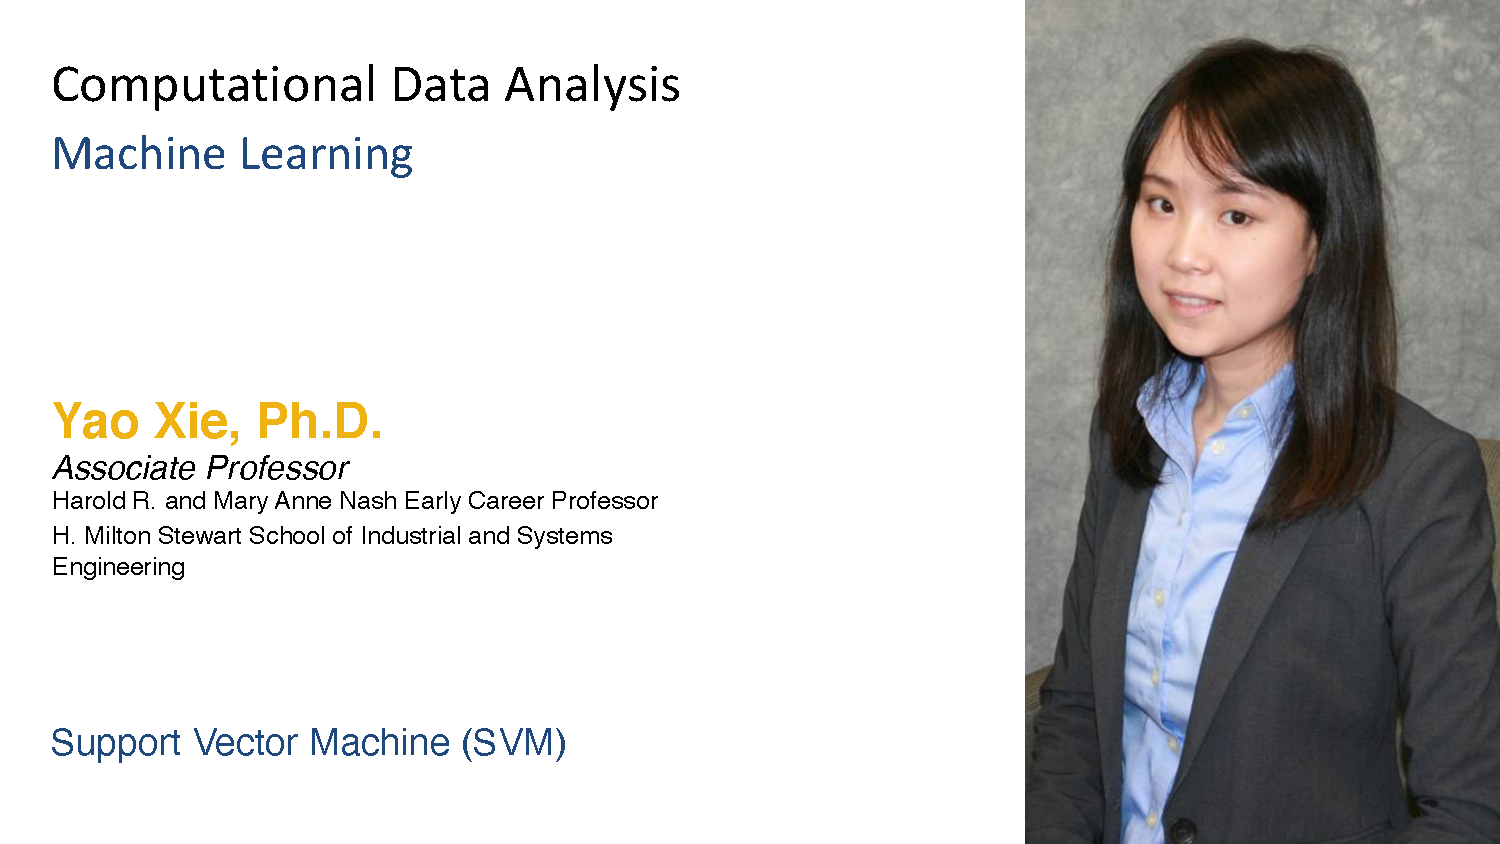
\includegraphics[width = 0.5\textwidth]{images/svm}
\end{center}

\begin{enumerate}
\item (10 points) For what range of parameter $h > 0$, the training points are still linearly separable?
\begin{tcolorbox}[breakable, enhanced]
\textbf{Solution:} The training points are linearly separable as long as the negative sample $x_3 = (h, 1)$ stays on the left hand side of the line $ y = x$ decided by the two positive samples $x_1 = (0,0)$ and $x_2 = (2,2)$. Therefore, for $h \in (0, 1)$, the training points are linearly separable.

\end{tcolorbox}

\item (10 points) Does the orientation of the maximum margin decision boundary change as $h$ changes, when the points are separable?
\begin{tcolorbox}[breakable, enhanced]
\textbf{Solution:} When $h$ changes between 0 and 1, the orientation of the maximum margin decision boundary dose not change. It will always be parallel to the line $ y = x$. As the two positive samples $x_1$ and $x_2$ will be on the margin, we have 
\begin{align*}
w_1 *0 + w_2 * 0 + b = 1, \\
w_1 * 2 + w_2 *2 + b = 1.
\end{align*} 
From the above equations we see $b=1$ and $w_1 + w_2 = 0.$ Therefore, the orientation of the maximum margin decision boundary will always be parallel to the vector $(1, 1)$.
\end{tcolorbox} 
\end{enumerate}


\end{enumerate}



\item {\bf Multi-class classification for MNIST data set, comparison.} (55 points)

This question is to compare different classifiers and their performance for multi-class classifications on the complete MNIST dataset at \url{http://yann.lecun.com/exdb/mnist/}. You can find the data file \textsf{mnist\_10digits.mat} in the homework folder. The MNIST database of handwritten digits has a training set of 60,000 examples, and a test set of 10,000 examples. We will compare {\bf KNN, logistic regression, SVM, kernel SVM, and  neural networks}. We suggest to use \textsf{Scikit-learn}, which is a commonly-used and powerful \textsf{Python} library with various machine learning tools. But you can also use other similar libraries in other programming languages of your choice to perform the tasks. Below are some tips. 

\begin{itemize}

\item We suggest you to ``standardize'' the features before training the classifiers, by dividing the values of the features by 255 (thus map the range of the features from [0, 255] to [0, 1]).

\item You may adjust the number of neighbors $K$ used in KNN to have a reasonable result (you may use cross validation but it is not required; any reasonable tuning to get good result is acceptable).

\item You may use a neural networks function \textsf{sklearn.neural\_network} with \textsf{hidden\_layer\_sizes = (20, 10)}. 

%Tune the step size so you have reasonable results. You may use \textsf{svc} and tune the penalty term $C$ to get reasonable results. 

\item For kernel SVM, you may use  radial basis function kernel, and a heuristic called ``median trick'': choose the parameter of the kernel $K(x, x') = \exp\{-\|x-x'\|^2/(2\sigma^2)\}$. Choose the bandwidth as $\sigma=\sqrt{M/2}$ where $M =$ the median of $\{\|x^i-x^j\|^2, 1\leq i, j \leq m', i\neq j \}$ for pairs of training samples. Here you can randomly choose $m'=1000$ samples from training data to use for the ``median trick''\footnote{Garreau, Damien, Wittawat Jitkrittum, and Motonobu Kanagawa. "Large sample analysis of the median heuristic." arXiv preprint arXiv:1707.07269 (2017).}.

\item For KNN and SVM, you can randomly downsample the training data to size $m=5000$, to improve computation efficiency. 
\end{itemize}

Train the classifiers on training dataset and evaluate on the test dataset.

\begin{enumerate}

	\item (50 points) Report confusion matrix, precision, recall, and F-1 score for each of the classifiers. For precision, recall, and F-1 score of each classifier, we will  need to report these for each of the digits. So you can create a table for this. For this question, each of the 5 classifier, {\bf KNN, logistic regression, SVM, kernel SVM, and  neural networks}, accounts for 10 points.
\begin{tcolorbox}[breakable, enhanced]
\textbf{Report:}
Firstly, we randomly sampled 5,000 examples from the 60,000 training examples for the purpose of shorter training time. Here is a histgram of the 10 classes in the downsampled training set. We can see that the classes are pretty balanced.\\
\begin{center}
\includegraphics[width=0.8\textwidth]{images/y_train.jpg}
\end{center}

Even though the training size is not very large, we still obtained pretty good classification accuracies on the 10,000 test data. 
We trained 5 classifiers using Sklearn and the accuracies ranges from 0.90 to 0.95. We will report on the five classifiers one by one and the confusion matrices of the results from each classifier is attached. Also, we listed and plotted the resulting precision, recall, and f1 score for each classifier on each class for easier comparison. 
\begin{itemize}
\newpage
\item KNN classifier: we find the best number of neighbors is 5 and the best distance function is $l2$ norm after applying GridSearchCV to search for number of neighbors from $1-9$ and distance functions from $l1$ norm and $l2$ norm. The resulting test accuracy from the best model is 0.93. It has very high recalls on class 0 and class 1. That means KNN classifier is did a good job on identifying 0s and 1s when it sees them. However, the precisions are not very high on these two classes, which means that the classifier incorrectly identified other numbers as 0s and 1s. From the confusion matrix, we see that KNN incorrectly classified 25 '2's as '0', 45 '2's as '1', and 44 '7's as '1'. Moreover, it also has difficulty in differentiating '4' and '9' as 67 '4's are classified as '9' and 25 '9's are classified as '4'.
\begin{center}
\begin{tabular}{| c | c | c | c | c | c | c | c |  c | c | c |}
\hline
KNN Classifer &  0 & 1 & 2 & 3 & 4 & 5 &  6 & 7 & 8 &  9  \\
\hline
Precision &  0.94 &  0.88 &  0.98 &  0.92 &  0.95 &  0.93 &  0.96 &  0.93 &  0.98 &  0.89 \\
\hline
Recall &  0.99 &  1.0 &  0.89 &  0.95 &  0.9 &  0.92 &  0.97 &  0.93 &  0.86 &  0.92 \\
\hline
F1 score &  0.96 &  0.94 &  0.93 &  0.93 &  0.92 &  0.93 &  0.96 &  0.93 &  0.92 &  0.9 \\
\hline
\end{tabular} 

\end{center}
\begin{center}
\includegraphics[width=0.9\textwidth]{images/cm_KNN.jpg}
\end{center}

\newpage
\item Logistic Regression: We fine tuned the regularization parameter $C$ from $\{0.1, 0.2, ..., 1.0\}$ and penalty function from $\{ \text{'l1', 'l2'}\}$ and found that the optimal $C = 0.2$ and optimal penalty is 'l2'. However, Logistic Regression has a less satisfying result compared to KNN classifier. This might due to the fact that the classes are not linearly separable while logistic regression can only has linear decision boundary. From here we can expect that the linear SVM should also has a not very satisfying result for the same reason. The confusion matrix shows that Logistic Regression is having difficulty in distinguishing '3' and '5', '4' and '9',  and '5' and '8'. Also, 38 '2's are classified as '8', and 36 '8's are classified as '3'.
\begin{center}
\begin{tabular}{| c | c | c | c | c | c | c | c |  c | c | c |}
\hline
Logistic Reg. &  0 & 1 & 2 & 3 & 4 & 5 &  6 & 7 & 8 &  9  \\
\hline
Precision &  0.94 &  0.95 &  0.93 &  0.87 &  0.89 &  0.88 &  0.93 &  0.93 &  0.85 &  0.87 \\
\hline
Recall &  0.98 &  0.97 &  0.87 &  0.9 &  0.92 &  0.83 &  0.95 &  0.9 &  0.84 &  0.87 \\
\hline
F1 score &  0.96 &  0.96 &  0.9 &  0.89 &  0.9 &  0.85 &  0.94 &  0.91 &  0.84 &  0.87 \\
\hline
\end{tabular} 

\end{center}
\includegraphics[width=0.9\textwidth]{images/cm_Log.jpg}

\newpage
\item SVM: Similar to Logistic Regression, we fine tuned the regularization parameter $C$ from $\{0.1, 0.2, ..., 1.0\}$ and penalty function from $\{ \text{'l1', 'l2'}\}$ and found that the optimal $C = 0.1$ and optimal penalty is 'l2'. The SVM has a very similar but slightly worse performance compared to Logistic Regression for the sake of nonlinearly separable data set and linear decision boundary. The confusion matrix shows that SVM is having difficulty in differentiating '3' and '5', '4' and '9',  '5' and '8', '7' and '9'. Also, 38 '2's are classified as '8', and 42 '8's are classified as '3'. The performance of SVM is very similar to Logistic Regression's performance. 

\begin{center}
\begin{tabular}{| c | c | c | c | c | c | c | c |  c | c | c |}
\hline
SVM &  0 & 1 & 2 & 3 & 4 & 5 &  6 & 7 & 8 &  9  \\
\hline
Precision &  0.92 &  0.96 &  0.92 &  0.87 &  0.89 &  0.84 &  0.93 &  0.92 &  0.84 &  0.87 \\
\hline
Recall &  0.97 &  0.97 &  0.86 &  0.88 &  0.91 &  0.84 &  0.92 &  0.9 &  0.81 &  0.87 \\
\hline
F1 score &  0.94 &  0.96 &  0.89 &  0.87 &  0.9 &  0.84 &  0.93 &  0.91 &  0.82 &  0.87 \\
\hline
\end{tabular} 

\end{center}
\includegraphics[width=0.9\textwidth]{images/cm_SVM.jpg}

\newpage
\item Kernel SVM: Before apply ``median trick'', the Kernel SVM did a slightly better job than linear SVM as the kernel trick allows for nonlinear decision boundaries. Then, we apply the ``median trick'' and found $M = 103.36$, which means $\sigma^2 = M/2 = 51.68$. The accuracy was greatly improved from $91\%$ to $95\%$. After that, we tuned the parameter $C$ from $\{1,2,...,14\}$ and found the optimal $C = 12$, which gives an accuracy of $96\%$. Large $C$ means that we do not allow many data to stay inside the margins. From the confusion matrix, we see that the most struggling thing for it is to distinguishing '4' and '9'. However, it is doing a much better job than the other models. 
\begin{center} 
\begin{tabular}{| c | c | c | c | c | c | c | c |  c | c | c |}
\hline
Kernel SVM &  0 & 1 & 2 & 3 & 4 & 5 &  6 & 7 & 8 &  9  \\
\hline
Precision & 0.96 &  0.98 &  0.96 &  0.94 &  0.95 &  0.94 &  0.96 &  0.97 &  0.95 &  0.95 \\
\hline
Recall & 0.99 &  0.99 &  0.95 &  0.96 &  0.97 &  0.96 &  0.97 &  0.94 &  0.93 &  0.92 \\
\hline
F1 score &  0.98 &  0.98 &  0.96 &  0.95 &  0.96 &  0.95 &  0.97 &  0.96 &  0.94 &  0.94 \\
\hline
\end{tabular} 

\end{center}

\includegraphics[width=0.9\textwidth]{images/cm_Ker.jpg}


\newpage 
\item Neural Network: We trained a 4-layer Neural Network with the first hidden layer of size 20 and second hidden layer of size 10. The performance is good. But not as good as Kernel SVM. Like other models, Neural Network is also struggling with differentiating '3' and '5', '3' and '8', '4' and '9'.  
\begin{center}
\begin{tabular}{| c | c | c | c | c | c | c | c |  c | c | c |}
\hline
Neural Network &  0 & 1 & 2 & 3 & 4 & 5 &  6 & 7 & 8 &  9  \\
\hline
Precision &  0.94 &  0.96 &  0.92 &  0.89 &  0.89 &  0.86 &  0.94 &  0.94 &  0.86 &  0.91 \\
\hline
Recall &  0.96 &  0.97 &  0.89 &  0.9 &  0.92 &  0.88 &  0.91 &  0.92 &  0.86 &  0.9 \\
\hline
F1 score &  0.95 &  0.97 &  0.91 &  0.89 &  0.91 &  0.87 &  0.92 &  0.93 &  0.86 &  0.91 \\
\hline
\end{tabular} 

\end{center}
\includegraphics[width=0.9\textwidth]{images/cm_Neu.jpg}

\end{itemize}

%\begin{center}
%Precision 
%
%\vspace{2 mm}
%\begin{tabular}{| c | c | c | c | c | c | c | c |  c | c | c |}
%\hline
%Classifiers &  0 & 1 & 2 & 3 & 4 & 5 &  6 & 7 & 8 &  9  \\
%\hline
%KNN classifier &  0.94 &  0.88 &  0.98 &  0.92 &  0.95 &  0.93 &  0.96 &  0.93 &  0.98 &  0.89 \\
%\hline
%Logistic Regressor &  0.94 &  0.95 &  0.93 &  0.87 &  0.89 &  0.88 &  0.93 &  0.93 &  0.85 &  0.87 \\
%\hline
%SVM &  0.92 &  0.96 &  0.92 &  0.87 &  0.89 &  0.84 &  0.93 &  0.92 &  0.84 &  0.87 \\
%\hline
%Kernel SVM &  0.96 &  0.97 &  0.94 &  0.93 &  0.93 &  0.94 &  0.96 &  0.96 &  0.94 &  0.93 \\
%\hline
%Neural Networks &  0.94 &  0.96 &  0.92 &  0.89 &  0.89 &  0.86 &  0.94 &  0.94 &  0.86 &  0.91 \\
%\hline
%\end{tabular} 
%
%\vspace{3 mm}
%
%Recall
%
%\vspace{2 mm}
%\begin{tabular}{| c | c | c | c | c | c | c | c |  c | c | c |}
%\hline
%Classifiers &  0 & 1 & 2 & 3 & 4 & 5 &  6 & 7 & 8 &  9  \\
%\hline
%KNN classifier &  0.99 &  1.0 &  0.89 &  0.95 &  0.9 &  0.92 &  0.97 &  0.93 &  0.86 &  0.92 \\
%\hline
%Logistic Regressor &  0.98 &  0.97 &  0.87 &  0.9 &  0.92 &  0.83 &  0.95 &  0.9 &  0.84 &  0.87 \\
%\hline
%SVM &  0.97 &  0.97 &  0.86 &  0.88 &  0.91 &  0.84 &  0.92 &  0.9 &  0.81 &  0.87 \\
%\hline
%Kernel SVM &  0.98 &  0.99 &  0.93 &  0.95 &  0.96 &  0.92 &  0.97 &  0.92 &  0.93 &  0.92 \\
%\hline
%Neural Networks &  0.96 &  0.97 &  0.89 &  0.9 &  0.92 &  0.88 &  0.91 &  0.92 &  0.86 &  0.9 \\
%\hline
%\end{tabular} 
%
%\vspace{3 mm}
%
%F1 Score
%
%\vspace{2 mm}
%\begin{tabular}{| c | c | c | c | c | c | c | c |  c | c | c |}
%\hline
%Classifiers &  0 & 1 & 2 & 3 & 4 & 5 &  6 & 7 & 8 &  9  \\
%\hline
%KNN classifier &  0.96 &  0.94 &  0.93 &  0.93 &  0.92 &  0.93 &  0.96 &  0.93 &  0.92 &  0.9 \\
%\hline
%Logistic Regressor &  0.96 &  0.96 &  0.9 &  0.89 &  0.9 &  0.85 &  0.94 &  0.91 &  0.84 &  0.87 \\
%\hline
%SVM &  0.94 &  0.96 &  0.89 &  0.87 &  0.9 &  0.84 &  0.93 &  0.91 &  0.82 &  0.87 \\
%\hline
%Kernel SVM &  0.97 &  0.98 &  0.94 &  0.94 &  0.95 &  0.93 &  0.96 &  0.94 &  0.93 &  0.93 \\
%\hline
%Neural Networks &  0.95 &  0.97 &  0.91 &  0.89 &  0.91 &  0.87 &  0.92 &  0.93 &  0.86 &  0.91 \\
%\hline
%\end{tabular} \end{center}

\end{tcolorbox}
\newpage
	\item (5 points) Comment on the performance of the classifier and give your explanation why some of them perform better than the others.	%\item (10 points) Plot the data points and decision boundary of each classifier. Comment on the difference between the decision boundary for the two classifiers. Please clearly represent the data points with different labels using different colors.
\begin{tcolorbox}[breakable, enhanced]
\textbf{Solution:}
We plotted the performance of the five classifiers for better comparison. From this 5,000 randomly sampled training set, our models gained the ability to distinguish different digits. From the plots we see that nonlinear models like Kernel SVM and KNN did a better job than linear models like Logistic Regression and SVM. The Neural Network has a performance in the middle. But if we add more training data and more hidden layers, I believe it will have a much better performance. \\
\includegraphics[width=0.325\textwidth]{images/Precision.jpg}
\includegraphics[width=0.325\textwidth]{images/Recall.jpg}
\includegraphics[width=0.325\textwidth]{images/F1-score.jpg}

\end{tcolorbox}
\end{enumerate}


\item {\bf Neural networks.} (Bonus: 10 points)

\begin{enumerate}
\item (2 points)
Consider a neural networks for a binary classification using sigmoid function for each unit. If the network has no hidden layer, explain why the model is equivalent to logistic regression. 
\begin{tcolorbox}[breakable, enhanced]
\textbf{Solution:} If the network has no hidden layer, then the loss function is $$l(w) = \sum_{i=1}^n (y^i - \sigma(w^Tx^i))^2.$$ This is exactly the loss function of logistic regression. 
\end{tcolorbox}

\item (8 points) 
Consider a simple two-layer network in the lecture slides. Given $m$ training data $(x^i, y^i)$, $i = 1, \ldots, m$, the cost function used to training the neural networks
\[
\ell(w, \alpha, \beta) = \sum_{i=1}^m (y^i - \sigma(w^T z^i))^2
\]
where $\sigma (x) = 1/(1+e^{-x})$ is the sigmoid function, $z^i$ is a two-dimensional vector such that  $z_1^i = \sigma(\alpha^T x^i)$, and $z_2^i = \sigma(\beta^T x^i)$. Show the that the gradient is given by
\[
\frac{\partial \ell(w, \alpha, \beta) }{\partial w}
= - \sum_{i=1}^m 2(y^i - \sigma(u^i))\sigma(u^i)(1-\sigma(u^i)) z^i,
\]
where $u^i = w^T z^i$. Also find the gradient of $\ell(w, \alpha, \beta)$ with respect to $\alpha$ and $\beta$ and write down their expression.
\begin{tcolorbox}[breakable, enhanced]
\textbf{Solution:} Note that $\frac{\partial \sigma(x)}{\partial x} = \sigma(x)(1-\sigma(x))$. Then by chain rule we have
\begin{align*}
\frac{\partial \ell(w, \alpha, \beta) }{\partial w}
& = \sum_{i=1}^m 2 (y^i - \sigma(w^Tz^i)) (-\sigma(w^Tz^i) (1 - (\sigma(w^Tz^i))) z^i)\\
& = -\sum_{i=1}^m 2(y^i - \sigma(u^i))\sigma(u^i)(1-\sigma(u^i)) z^i 
\end{align*}
with $u^i = w^T z^i$. Similarly we have 
\begin{align*}
\frac{\partial \ell(w, \alpha, \beta) }{\partial \alpha}
& = \frac{\partial \ell}{\partial z_1^i} \frac{\partial z_1^i} {\partial \alpha} \\
& = \left (-\sum_{i=1}^m 2(y^i - \sigma(u^i))\sigma(u^i)(1-\sigma(u^i)) w_1 \right )\left( \sigma(\alpha^T x^i) (1 - \sigma(\alpha^T x^i)) x^i \right )\\
& = -\sum_{i=1}^m 2(y^i - \sigma(u^i))\sigma(u^i)(1-\sigma(u^i)) w_1 \sigma(\alpha^T x^i) (1 - \sigma(\alpha^T x^i)) x^i 
\end{align*}
and 
\begin{align*}
\frac{\partial \ell(w, \alpha, \beta) }{\partial \beta}
& = \frac{\partial \ell}{\partial z_2^i} \frac{\partial z_2^i} {\partial \beta} \\
& = \left (-\sum_{i=1}^m 2(y^i - \sigma(u^i))\sigma(u^i)(1-\sigma(u^i)) w_2 \right )\left( \sigma(\beta^T x^i) (1 - \sigma(\beta^T x^i)) x^i \right )\\
& = -\sum_{i=1}^m 2(y^i - \sigma(u^i))\sigma(u^i)(1-\sigma(u^i)) w_2 \sigma(\beta^T x^i) (1 - \sigma(\beta^T x^i)) x^i,
\end{align*}
where $w^T = (w_1, w_2)$.
\end{tcolorbox}
\end{enumerate}


\end{enumerate}





\end{document}
